\section{Lissajous-based exhibits}
Lissajous figures (named after the 19th century French mathematician Jules Antoine Lissajous) are curves determined by the intersection of two perpendicular oscillating movements. Mathematically, their coordinates $x,y$ in the plane are given for each time $t$ by the formulas
$$\left\{ \begin{array}{rcl}
x &=& \sin(a\cdot t) \\
y &=& \sin(b\cdot t + \varphi)
\end{array} \right. $$
where $t$ is the time parameter (angle),  $a$ and $b$ are the two frequencies, and $\varphi$ is the phase shift between one and the other. For different values of the time $t$, the equations trace a curve inside a square. Its shape depends essentially on the numerical ratio of the two frequencies. If $a=b$, or $a/b=1$, then the figure closes after one period and the result is a line or an ellipse. If $a/b = 3/2$, the curve closes after $3\cdot 2=6$ cycles and is quite clean. In general, ratios of small numbers make simple curves. On the contrary, if the values are in more complex ratios such as $a/b = 23/22$, the curve closes after many cycles ($22\cdot 23=506$ cycles) and the figure is more dense and messy. Thus, Lissajous figures are a tool to visualize when two numbers are in a simple ratio.

Here our oscillations are sound, and the frequency of the sound is perceived as pitch in our ears. In music, a fundamental idea tracing back to Pythagoras, is that sounds with frequencies in small number ratios sound consonant together, and frequencies with more complicated number ratios are less consonant. This is why Lissajous figures are used to visualize consonance or dissonance. Classical consonant intervals are the octave (ratio 2:1), the Fifth (ratio 3:2) and the Major Third (5:4).

It is also possible to have three-dimensional Lissajous curves, just analogous to the flat ones, but with three perpendicular vibrations instead of two. Three notes playing together form a triad chord, which are the base for music composition. In the just intonation tuning, major chords are notes in ratios 4:5:6, minor chords in ratios 10:12:15, and so on.

Remarkably, these arithmetic relations produce in us feelings as ``happy'' for major chords, ``sad'' for minors,
``tense'', ``cozy'', etc. although a real mastery is needed to compose a piece that successfully conveys emotions.

\section{Lissajous gallery}
The six pictures here are an artistic representation of Lissajous figures. To create them, the artist Ryan Cashman starts with a curve in space defined by two sinusoidal waves, that is, a Lissajous figure, but also modulated by a second oscillation. With the chosen frequency ratios, the curve drifts from itself passing close but not exactly over itself. The program calculates points at regular intervals along the curve, creating vertices. The vertices are connected in order to create the base curve of the shape. Then additional lines are drawn between any pair of vertices located close enough in the space, to form a web like representation of a surface. The frequencies chosen for each pictures are those from musical chords in the standard equal tempered tuning.

Mathematically, the $x$ (horizontal) and $y$ (vertical) position of each vertex is calculated with the formula
$$\left\{ \begin{array}{rcl}
x &=& \sin(f_X\cdot t + \varphi) \cdot \cos(m_X \cdot t) \\
y &=& \sin(f_Y\cdot t + \varphi) \cdot \cos(m_Y \cdot t)
\end{array} \right. $$
where additionally we have $m_X$ and $m_Y$ as modulation coefficients.


\begin{figure}[!h]
\centering
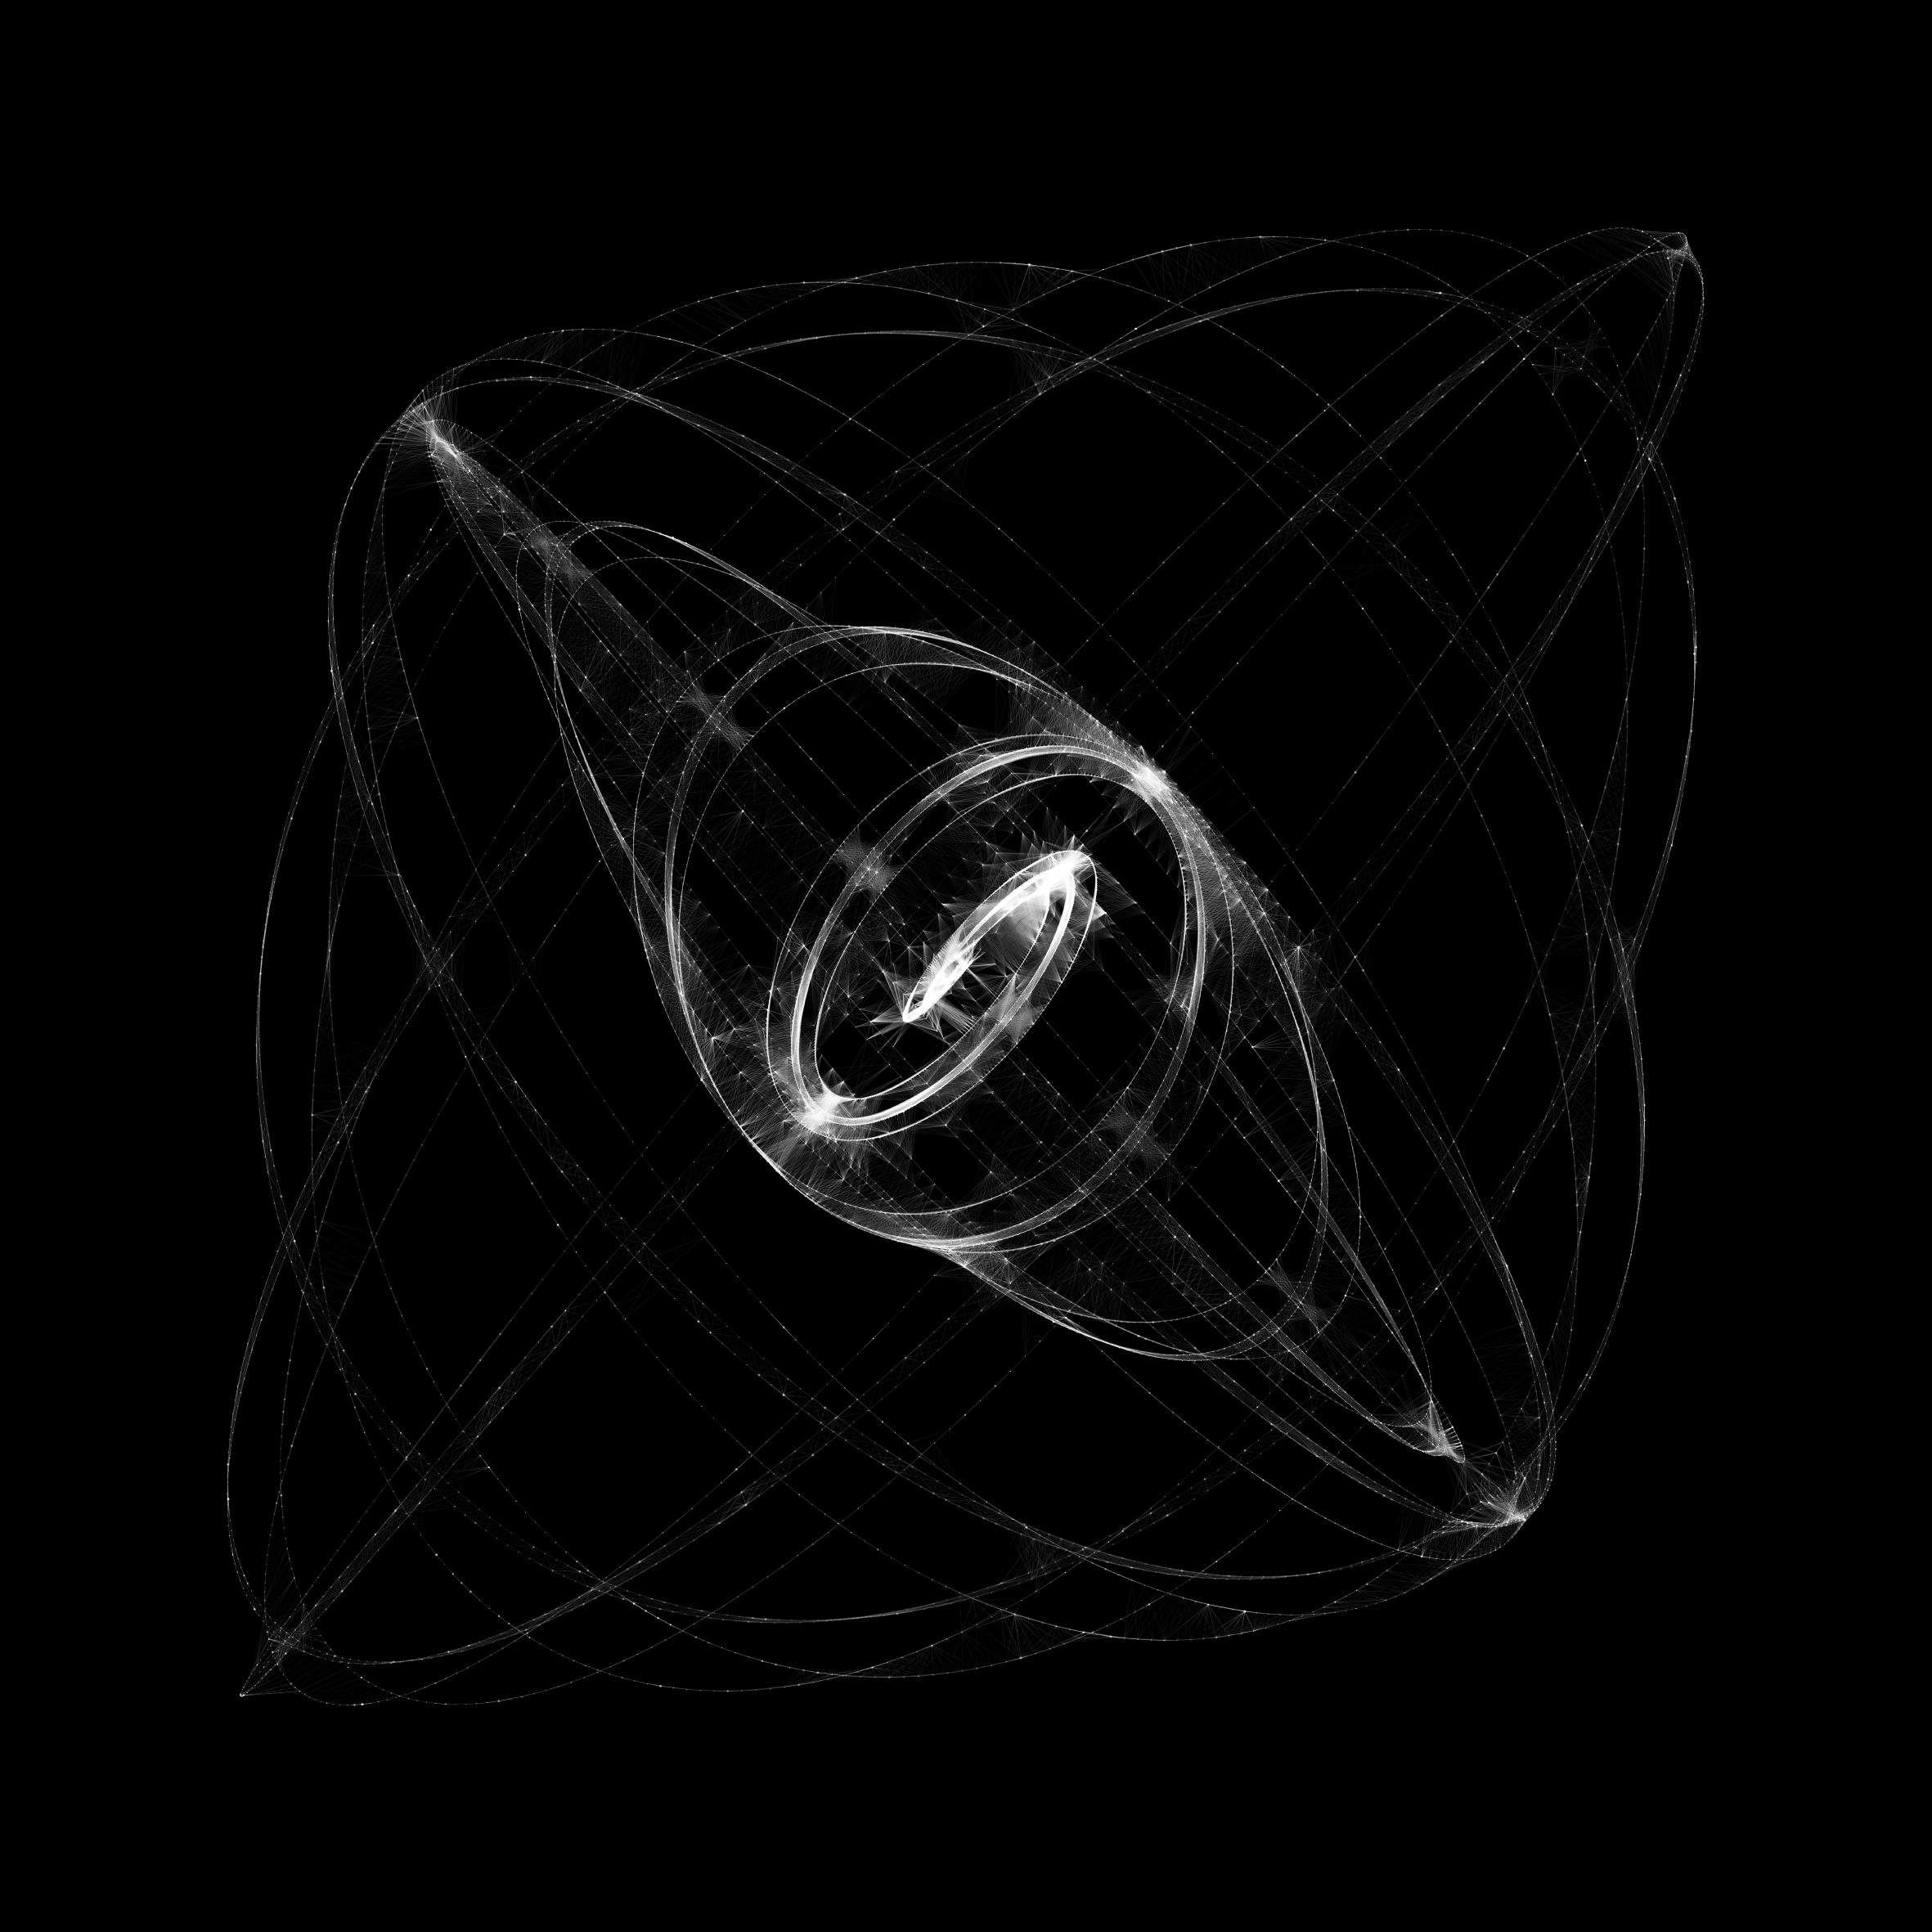
\includegraphics[width=0.6\textwidth]{Lissajous_Cashman}
\caption*{Major second.}
\end{figure}


\begin{sectcredits}
\item[Author of the gallery:] Ryan Cashman.
\item[Text:] Ryan Cashman.
\end{sectcredits}

\section{The Harmonic Series}
When Jules Antoine Lissajous invented the device that produces the curves named after him, it was with the purpose of standardizing musical sound. In his original design, two tuning forks are placed perpendicularly, each with a mirror attached to its tip. A beam of light is directed to the first mirror, reflected to the second one and finally to a screen. If the frequencies of the tuning forks are related by simple integer ratios, which make them harmonious musically, the figures are harmonious visually as well.

\begin{figure}[!h]
\centering
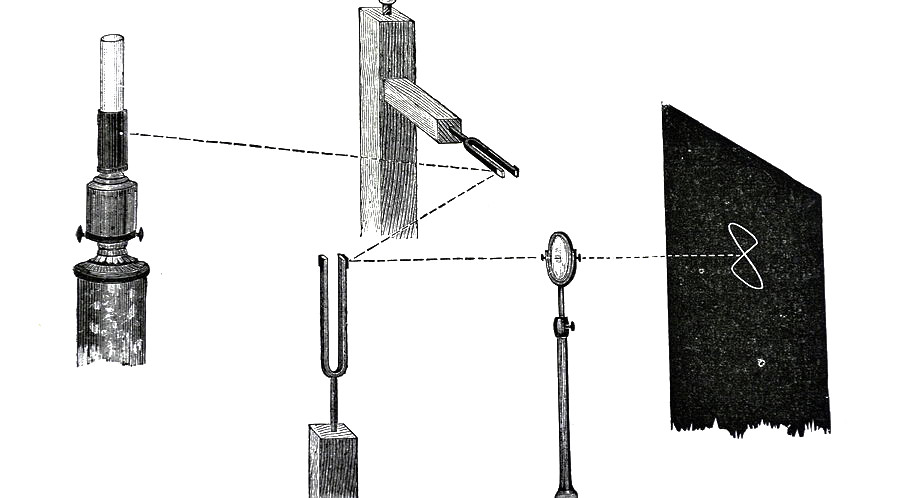
\includegraphics[width=0.6\textwidth]{Lissajous_apparatus}
\end{figure}


The pieces in this series by artists Manuela Donoso and Luisa Pereira re-create and extend Lissajous' device using contemporary technology, bringing it from the realm of the functional into the realm of interactive art. Their devices invite us to use our voices to interact with sound vibrations visually, and develop a deeper, intuitive understanding of the interplay between noise, consonance, dissonance, and harmony.



\subsection{Device \#1}
Microphones, amplifiers, speakers, mirrors, laser.

This device adds interactivity to Lissajous' original apparatus by replacing Lissajous tuning forks with two speakers, and the light source with a laser pointer. Each speaker is connected to a microphone, and the two mirrors attached to their membranes vibrate in perpendicular directions. As the speakers vibrate with the voices of visitors, the projected figures evolve: percussive sounds generate chaotic figures, dissonant intervals generate messy figures, consonant intervals generate harmonious figures. Whistling will result in sharper curves than singing the same notes, hinting at the variety and richness of timbre in music.

\subsection{Device \#2}
Microphone, amplifier, A/D converter, micro-controller, synthesizers, holographic display.

This device adds a third dimension to Lissajous figures, allowing for the visualization of triadic chords -- that is, chords composed by three notes. The first and second vibrations are notes produced by synthesizers; visitors can change their pitches by moving sliders up and down. The third vibration is input by visitors through a microphone: they can sing varying pitches, talk, speak, or experiment with any sound they like. The custom software plots these three vibrations onto 3D space over time: the first synthesizer determines the x, the voice the y, and the second synthesizer the z position of each point in the resulting 3D figure. The figure is then encoded to be rendered onto a holographic display (``The Looking Glass''), creating an ever-evolving sculpture of light.

\subsection{Triad Sculptures}
3D stereolithography prints.

Three-dimensional Lissajous figures represent three different triads: Major (with frequency ratios of $4:5:6$), Minor ($10:12:15$), and Diminished (approximately $20:24:29$). Observe that in both the Major and the Minor cases, when we take pairs of frequencies they are in ratios $4:5$, $5:6$, and $2:3$, but the Lissajous figures (and the chords) are not the same. You can use one of the bright light focus to cast a shadow. The number of lobes on each side of the flat Lissajous figures give you the ratios.

These figures can be reproduced by having Device \#2 receive pitches at these ratios, by singing and shifting the synthesizer sliders.

\begin{sectcredits}

\item[Authors of the series:] Manuela Donoso and Luisa Pereira.\\
Production (Device \#1): Manuela Donoso and Lukas Reck for IMAGINARY.\\
Programming (Device \#2): Luisa Pereira and Ricardo Dodds.

\item[Sponsored:] 3D holographic display by The Looking Glass \\
\url{https://lookingglassfactory.com}.

\item[Text:] Manuela Donoso and Luisa Pereira.

\item[References:] \strut \\
\url{www.theharmonicseries.net}

\end{sectcredits}
